\documentclass[12pt]{article}
\usepackage[english]{babel}
\usepackage{graphicx}
\usepackage[utf8]{inputenc}
\usepackage{blindtext} % Package to generate dummy text throughout this template 

\usepackage[sc]{mathpazo} % Use the Palatino font
\usepackage[T1]{fontenc} % Use 8-bit encoding that has 256 glyphs
\linespread{1.05} % Line spacing - Palatino needs more space between lines
\usepackage{microtype} % Slightly tweak font spacing for aesthetics

\usepackage[english]{babel} % Language hyphenation and typographical rules

\usepackage[hmarginratio=1:1,top=32mm,columnsep=20pt]{geometry} % Document margins
\usepackage[hang, small,labelfont=bf,up,textfont=it,up]{caption} % Custom captions under/above floats in tables or figures
\usepackage{booktabs} % Horizontal rules in tables

\usepackage{lettrine} % The lettrine is the first enlarged letter at the beginning of the text

\usepackage{enumitem} % Customized lists
\setlist[itemize]{noitemsep} % Make itemize lists more compact

\usepackage{abstract} % Allows abstract customization
\renewcommand{\abstractnamefont}{\normalfont\bfseries} % Set the "Abstract" text to bold
\renewcommand{\abstracttextfont}{\normalfont\small\itshape} % Set the abstract itself to small italic text

\usepackage{titlesec} % Allows customization of titles
\renewcommand\thesection{\Roman{section}} % Roman numerals for the sections
\renewcommand\thesubsection{\roman{subsection}} % roman numerals for subsections
\titleformat{\section}[block]{\large\scshape\centering}{\thesection.}{1em}{} % Change the look of the section titles
\titleformat{\subsection}[block]{\large}{\thesubsection.}{1em}{} % Change the look of the section titles

\usepackage{fancyhdr} % Headers and footers
\pagestyle{fancy} % All pages have headers and footers
\fancyhead{} % Blank out the default header
\fancyfoot{} % Blank out the default footer
\fancyhead[C]{My first scientific paper $\bullet$ 2022 $\bullet$ MIPT} % Custom header text
\fancyfoot[RO,LE]{\thepage} % Custom footer text

\usepackage{titling} % Customizing the title section

\usepackage{hyperref} % For hyperlinks in the PDF
\usepackage{amssymb,amsmath,amsthm}

\theoremstyle{plain}
\newtheorem{proposition}{Proposition}
\theoremstyle{definition}
\newtheorem{definition}{Definition}
\newtheorem{notation}{Notation}
\newtheorem{example}{Example}
\DeclareMathOperator{\sign}{sign}

\setlength{\droptitle}{-4\baselineskip} % Move the title up

% Keywords command
\providecommand{\keywords}[1]
{
  \small	
  \textbf{\textit{Keywords}} #1
}

\title{\textbf{\Huge{Machine learning approach to startup success prediction}}}
\author{%
\textsc{Pavlov D.} \\[1ex] 
\normalsize MIPT\\ 
\normalsize \href{mailto:dima-pavlov@phystech.edu}{dima-pavlov@phystech.edu}
\and 
\textsc{Moiseev A.} \\[1ex] 
\normalsize MIPT
}

\date{\today}

\renewcommand{\maketitlehookd}{

\begin{abstract}
% - wide-range field of the investigated problem,
% - narrow problem to focus on,
% - features and conditions of the problem,
% - the novelty (please not exaggerate),
% - application to illustrate with (put the results here later).

This paper deals with a model for predicting the success of startups based on data about companies from CrunchBase and data about founders and investors associated with the company from LinkedIn. Unlike CrunchBase, where we have data with a clear structure, in a social network, data is filled in in the free form. In the last decade, natural language processing has shown good results when working with unstructured data. The approach for model construction using data about founders is new for the venture industry.
\noindent  \\

\keywords{Venture Capital · Unsupervised learning · Natural language processing}

\end{abstract}

}

\begin{document}

\maketitle

\clearpage

\section{Introduction}

% - the research goal (and its motivations),
% - the object of research (introduce main termini),
% - the problem (what is the challenge),
% - methodology: literature review and state-of-the-art
% - the project tasks,
% - the proposed solution, its novelty and advantages,
% - the profs and cons of recent works,
% - goal of the experiment, set up, data sets, workflow.

%There is a lot of unstructured information on the Internet that is useful for people who are professionally-looking for new projects and ideas. Data mining in venture business allows to collect big data usefull for prediction models from social networks and news. 

The number of startups born every day is growing from year to year. 
The growth leads to an increase in the load on the pipeline of a venture capital company. 
These companies are investing in the development of scoring models of startups to reduce the load on their pipelines. 
The scoring models summarize the experience of a venture analyst and automate routines such as reviewing reports and information about received investment rounds. %CrunchBase
However, in this industry, not only technical indicators are important, but also the network of people working on projects. 
The network consists of information that gets into social networks and news. 
At the moment, only human can process this information qualitatively. 
This is the difficulty that models for predicting the success of startups face. 

The goal of the authors was to build a model for predicting the success of a startup using CrunchBase and LinkedIn data. 
The model uses unstructured data clustered according to their meaning.

\section{Problem statement}

%Describe the elements of your problem statement:
% - the sample set,
% - its origin, or its algebraic structure,
% - statistical hypotheses of data generation,
% - [conditions of measurements] ,
% - [restrictions of the sample set and its values],
% - your model in the class of models,
% - restrictions on the class of models,
% - the error function (and its inference) or a loss function, or a quality criterion,
% - cross-validation procedure,
% - restrictions to the solutions,
% - external (industrial) quality criteria,
% - the optimization statement as argmin
%Define the main termini: what is called the model, the solution, the algorithm.

%Note that:

% - The model is a parametric family of functions to map design space to target space.
% - The criterion (error function) is a function to optimize in order to obtain an optimal solution (model parameters, a function).
% - The algorithm transforms solution space, usually iteratively.
% - The method combines a model, a criterion, and an algorithm to produce a solution.
%Check it:

% - the regression model,
% - the sum of squared errors,
% - the Newton-Raphson algorithm,
% - the method of least squares.

1

\section{Computational experiment}

The task is to build a model for prediction the success of a startup. This task is decomposed into several subtasks:

\begin{enumerate}
    \item Collect the data from CrunchBase and LinkedIn
    \item Preprocess data
    \item Create a model
\end{enumerate}

The key issue in this workfow is data preprocesing. As mentioned earlier, the novelty of the model in the use of unstructured data from social networks. 

<ToDo sample of data and show the problem>

Therefore, in the article we will focus on building an informational description of people's backgrounds from unstructured data. Our goal is to group people according to each of the available features:

\begin{itemize}
    \item Education field of study
    \item Profession skills
    \item Academic degree
    \item Work experience
\end{itemize}

\subsection{Data collection}

Data from CrunchBase has this structure: ...<todo scheme describe>

Data from LinkedIn has Json structure: ...<todo scheme describe>


\subsection{Data preprocessing}

Data from LinkedIn is processed using clustering and embeddings obtained using a neural network based on BERT: LaBSE (todo link to huggingface). The clustering is carried out using the kMeans algorithm.

\subsection{Model building}

\section{Results}

\subsection{Preprocess data}

<Show Word2Vec property of embeddings>

We can see that it turns out that the objects fall into clusters, but sometimes the clusters overlap. This is because TSNE transforms 754 dimensional space into 2 dimensional space. 

\begin{figure}[!h]
  \centering
  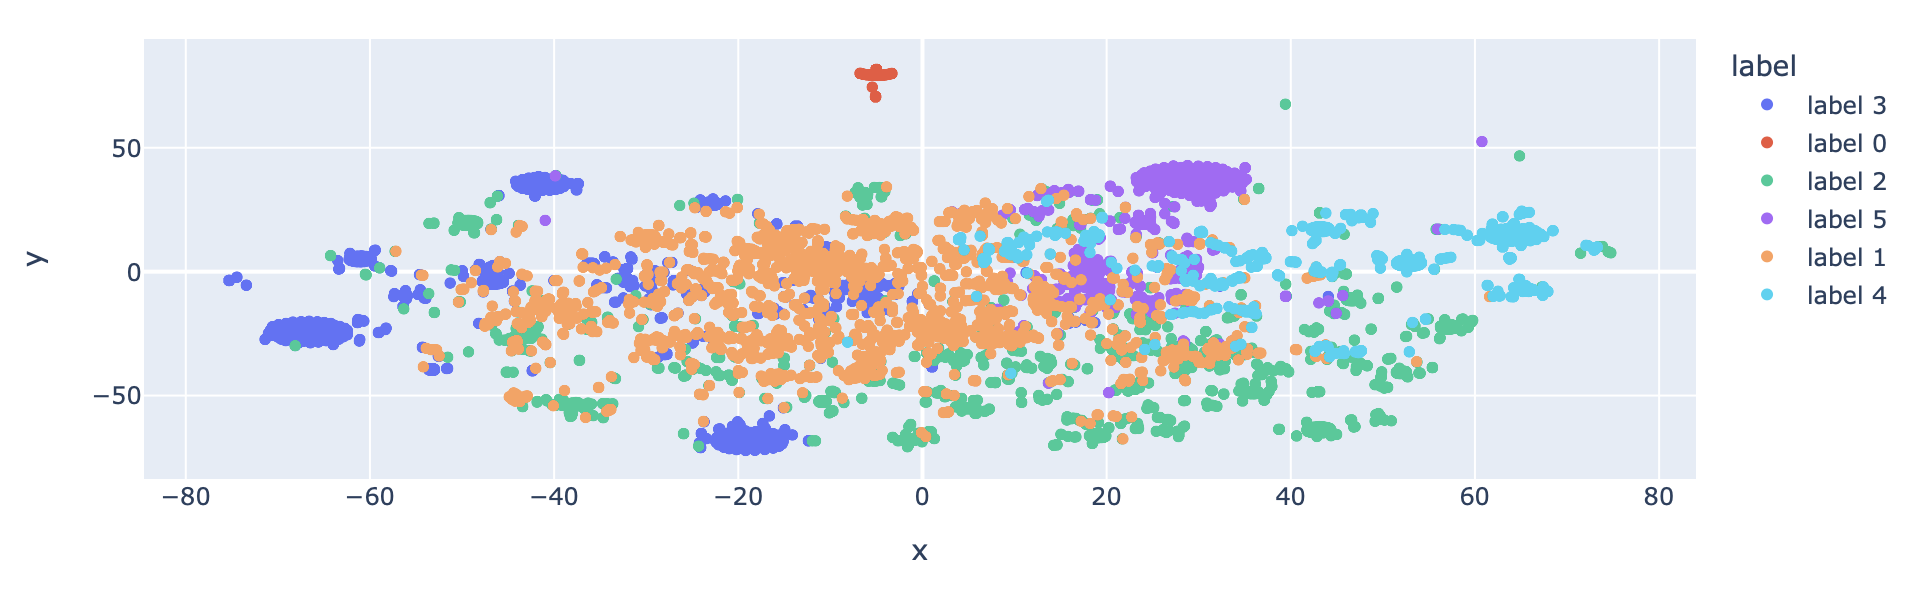
\includegraphics[width=160mm]{figures/paper/kMeans-9_03.png}
  \label{fig:gd}
  \caption{Education field of study clustering}
\end{figure}

The clustering coefficient -- Silhouette  metric is $0.26$, which indicates that clusters are more likely to be allocated than not.

\end{document}